\documentclass[xga]{xdvislides}
\usepackage[landscape]{geometry}
\usepackage{array}
\usepackage{graphics}
\usepackage{graphicx}
\usepackage{colordvi}
\usepackage{tabularx}
\usepackage{multirow}
\usepackage{fancyvrb}

\fvset{fontfamily=courier,commandchars=\\\{\}}

\newcommand{\smallish}{\fontsize{16}{16}\selectfont}

\begin{document}
\setfontphv

%%% Headers and footers
\lhead{\slidetitle}				% default:\lhead{\slidetitle}
\chead{CS615 - Aspects of System Administration}% default:\chead{\relax}
\rhead{Slide \thepage}				% default:\rhead{\sectiontitle}
\lfoot{\Gray{Review}}% default:\lfoot{\slideauthor}
\cfoot{\relax}					% default:\cfoot{\relax}
\rfoot{\Gray{\today}}

\vspace*{\fill}
\begin{center}
	\Hugesize
		CS615 - Aspects of System Administration\\ [1em]
		The Whole Semester In One Class\\ [1em]
	\hspace*{5mm}\blueline\\ [1em]
	\Normalsize
		Department of Computer Science\\
		Stevens Institute of Technology\\
		Jan Schaumann\\
		\verb+jschauma@stevens.edu+ \\
		\verb+http://www.cs.stevens.edu/~jschauma/615A/+
\end{center}
\vspace*{\fill}
%\setcounter{page}{0}
%\clearpage

\subsection{Basic Disk Concepts: Storage Models}
Direct Attached Storage (DAS)
\vfill
\begin{center}
	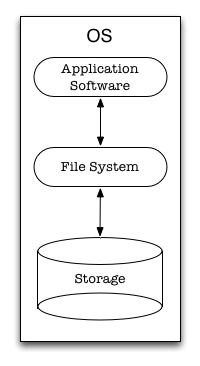
\includegraphics[scale=0.8]{pics/das.eps} \\
\end{center}
\verb+ssh lab 'df -hT /'+
\vfill

\subsection{Basic Disk Concepts: Storage Models}
Network Attached Storage (NAS)
\vfill
\begin{center}
	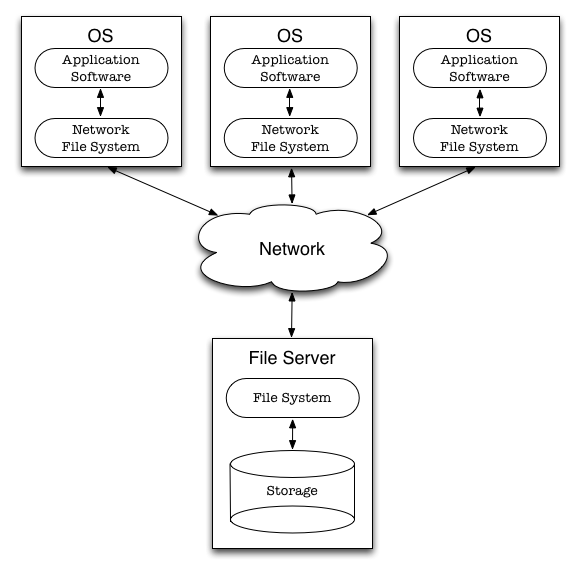
\includegraphics[scale=0.5]{pics/nas.eps} \\
\end{center}
\verb+ssh lab 'df -hT /home/$(whoami)'+
\vfill

\subsection{Basic Disk Concepts: Storage Models}
Storage Area Networks (SAN)
\vfill
\begin{center}
	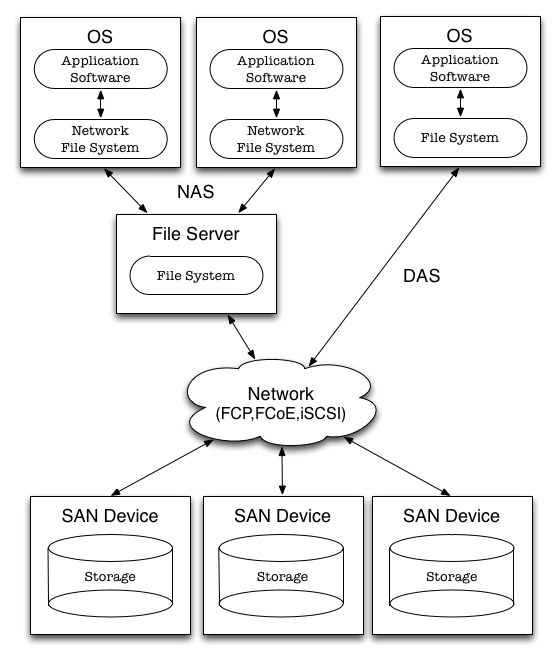
\includegraphics[scale=0.5]{pics/san-nas-das.eps} \\
\end{center}
\vfill

\subsection{Basic Disk Concepts: Storage Models}
Cloud Storage (Examples: EBS, S3)
\vfill
\begin{center}
	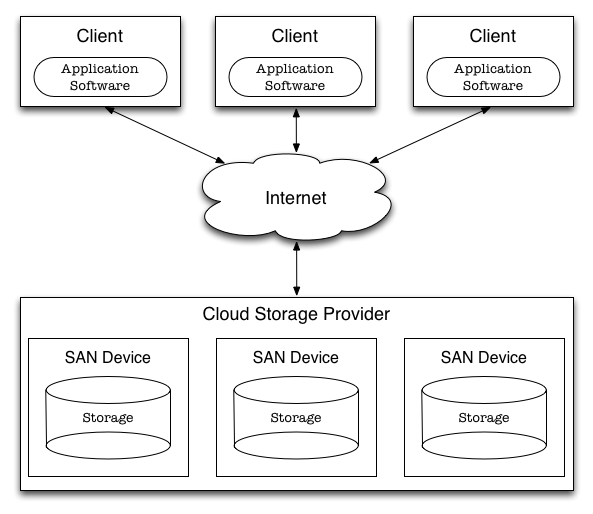
\includegraphics[scale=0.6]{pics/cloud-storage.eps} \\
\end{center}
\vfill

\subsection{Basic Disk Concepts: Disk Devices}
\vfill
	\begin{center}
		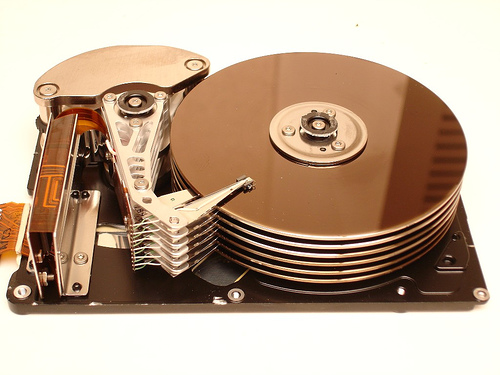
\includegraphics[scale=0.9]{pics/6platter.eps} \\
	\end{center}
\vfill

\subsection{Basic Disk Concepts: Physical Disk Structure}
\vfill
	\begin{center}
		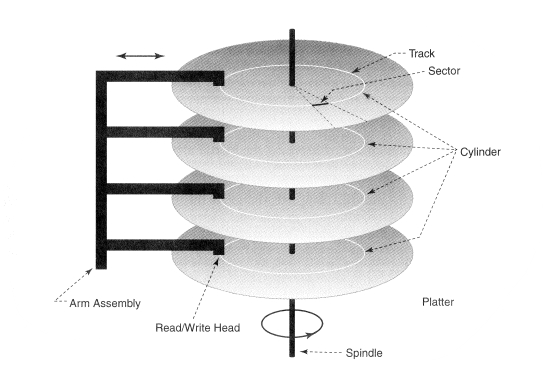
\includegraphics[scale=1.2]{pics/cylinders.eps} \\
	\end{center}
\vfill

\subsection{Basic Disk Concepts: Partitions}
NetBSD example (from {\tt disklabel(8)})

\begin{tabular}{ l l c }
Partition 'a': & / & \\
Partition 'b': & swap & \\
Partition 'e': & /home & \\
\end{tabular}

\begin{verbatim}
#        size    offset   fstype [fsize bsize cpg/sgs]
a:  20972385        63   4.2BSD   4096 32768  1180  # (Cyl.      0*- 20805)
b:   1048320  20972448     swap                     # (Cyl.  20806 - 21845)
c:  78140097        63   unused      0     0        # (Cyl.      0*- 77519)
d:  78140160         0   unused      0     0        # (Cyl.      0 - 77519)
e:  56119392  22020768   4.2BSD   4096 32768 58528  # (Cyl.  21846 - 77519)
\end{verbatim}

\subsection{Basic Filesystem Concepts: The UNIX Filesystem}
\vspace*{\fill}
\begin{center}
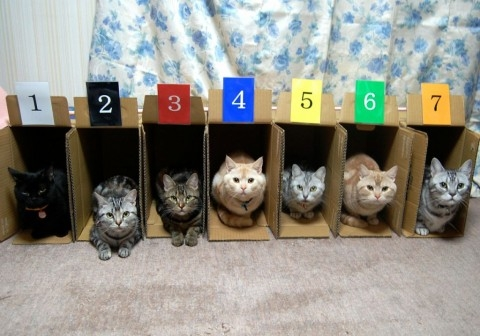
\includegraphics[scale=1.0]{pics/numbered-cats.eps} \\
\end{center}
\vspace*{\fill}

\subsection{Basic Filesystem Concepts: The UNIX Filesystem}
The filesystem is responsible for storing the data on the disk.
So to read/write data, it needs to know in which physical blocks the actual
data is located; ie how to map files to the disk blocks.
\\

Components of the Berkeley Fast Filesystem:
\\

\newcolumntype{S}{>{\centering\arraybackslash} m{.4\linewidth} }
\begin{tabular}{ p{10cm} S }
\begin{itemize}
	\item set of {\em inode} storage cells
\end{itemize}
{\tt df -i}
& \multirow{2}{*}{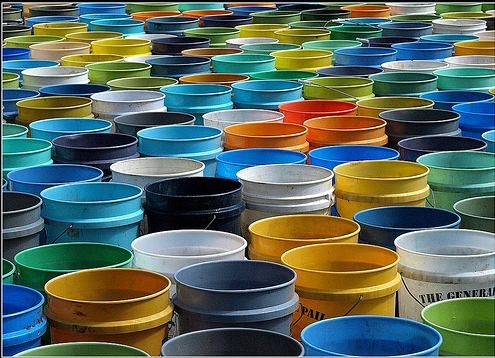
\includegraphics[scale=0.5]{pics/buckets.eps}} \\
\end{tabular}

\subsection{Basic Filesystem Concepts: The UNIX Filesystem}
The filesystem is responsible for storing the data on the disk.
So to read/write data, it needs to know in which physical blocks the actual
data is located; ie how to map files to the disk blocks.
\\

Components of the Berkeley Fast Filesystem:
\\

\begin{tabular}{ p{10cm} S }
\begin{itemize}
	\item set of {\em inode} storage cells
	\item set of scattered ``superblocks''
\end{itemize}
{\tt newfs -N /dev/rdsk/c1t2160d0s0}
& \multirow{2}{*}{
\includegraphics[scale=0.3]{pics/lego.eps}} \\
\end{tabular}

\subsection{Basic Filesystem Concepts: The UNIX Filesystem}
The filesystem is responsible for storing the data on the disk.
So to read/write data, it needs to know in which physical blocks the actual
data is located; ie how to map files to the disk blocks.
\\

Components of the Berkeley Fast Filesystem:
\\

\begin{tabular}{ p{10cm} S }
\begin{itemize}
	\item set of {\em inode} storage cells
	\item set of scattered ``superblocks''
	\item map of disk blocks
\end{itemize}
& \multirow{2}{*}{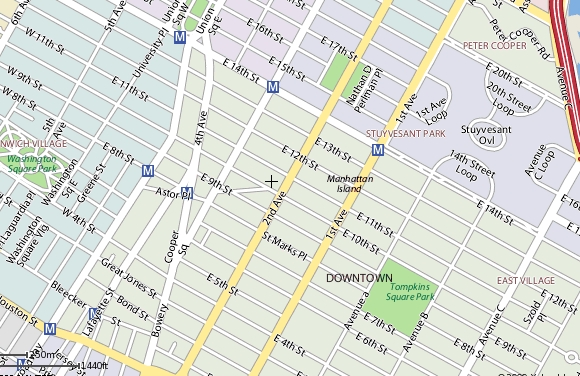
\includegraphics[scale=0.5]{pics/map.eps}} \\
\end{tabular}

\subsection{Basic Filesystem Concepts: The UNIX Filesystem}
The filesystem is responsible for storing the data on the disk.
So to read/write data, it needs to know in which physical blocks the actual
data is located; ie how to map files to the disk blocks.
\\

Components of the Berkeley Fast Filesystem:
\\

\begin{tabular}{ p{10cm} S }
\begin{itemize}
	\item set of {\em inode} storage cells
	\item set of scattered ``superblocks''
	\item map of disk blocks
	\item block usage summary
\end{itemize}
{\tt fstyp -v /dev/rdsk/c1t2160d0s0  | more}
& \multirow{2}{*}{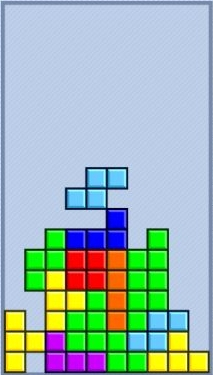
\includegraphics[scale=0.5]{pics/tetris.eps}} \\
\end{tabular}

\subsection{Basic Filesystem Concepts: The UNIX Filesystem}
The filesystem is responsible for storing the data on the disk.
So to read/write data, it needs to know in which physical blocks the actual
data is located; ie how to map files to the disk blocks.
\\

Components of the Berkeley Fast Filesystem:
\\

\begin{tabular}{ p{10cm} S }
\begin{itemize}
	\item set of {\em inode} storage cells
	\item set of scattered ``superblocks''
	\item map of disk blocks
	\item block usage summary
	\item set of data blocks
\end{itemize}
& \multirow{2}{*}{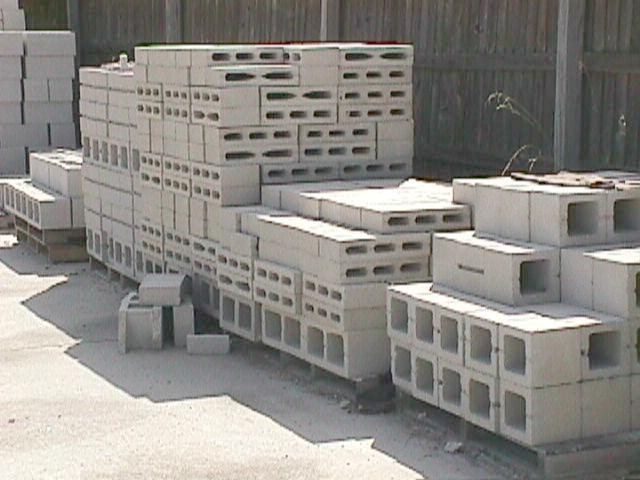
\includegraphics[scale=0.3]{pics/block.eps}} \\
\end{tabular}

\subsection{Basic Filesystem Concepts: The UNIX Filesystem}
\begin{center}
	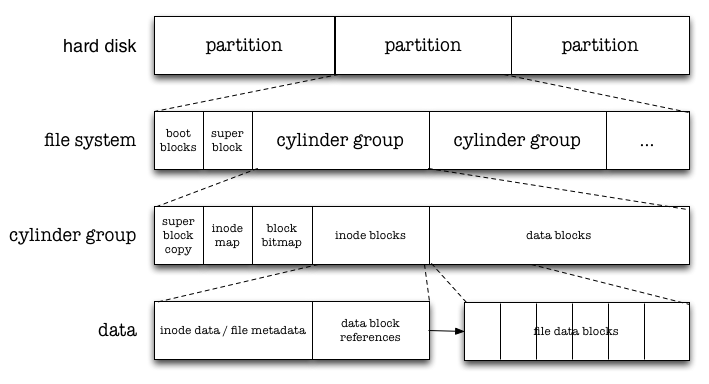
\includegraphics[scale=0.8]{pics/ufs-details.eps} \\
\end{center}
\vspace*{\fill}

\subsection{Basic Filesystem Concepts: The UNIX Filesystem}
Information stored in an {\em inode}:
\begin{itemize}
	\item user owner and group owner ID's
	\item file type
	\item access mode (permissions)
	\item file access and modification time
	\item file status modification time
	\item number of links to the file
	\item size of the file
	\item disk device containing this file
\end{itemize}

\begin{verbatim}
$ stat /etc/passwd
\end{verbatim}

\newpage
\vspace*{\fill}
\begin{center}
    \Hugesize
        Presentation \\ [1em]
    \hspace*{5mm}
    \blueline\\
    \hspace*{5mm}\\
	Sonal Mehta
\end{center}
\vspace*{\fill}


\newpage
\vspace*{\fill}
\begin{center}
    \Hugesize
        Lecture 03 \\ [1em]
    \hspace*{5mm}
    \blueline\\
    \hspace*{5mm}\\
	Software Installation Concepts
\end{center}
\vspace*{\fill}

\subsection{Down the stack we go}
Consider a website on an AWS EC2 instance...
\\

...it might:

\begin{itemize}
	\item require PHP, Perl, Ruby, Javascript, ...
	\item which uses generic library functions
	\item which make various system calls
	\item which the kernel handles for the OS
	\item which is running in a virtual machine
	\item which is running on top of a hypervisor
	\item which uses firmware to manage various components
	\item which is running on some hardware
\end{itemize}


\subsection{...and back up again}
Bringin up this web service might include...
\\

\begin{itemize}
	\item power on hardware
	\item POST and other firmware initialization
	\item first stage boot loader
	\item second stage boot loader
	\item hypervisor kernel dom0 starts
	\item domU is started
	\item guest OS kernel starts
	\item kernel initializes (virtual) hardware
	\item {\tt init(8)} (or similar) starts
	\item system processes / daemons start
	\item web server runs, binds network socket, serves content
\end{itemize}

\subsection{Types of Software}
\vfill
\begin{center}
	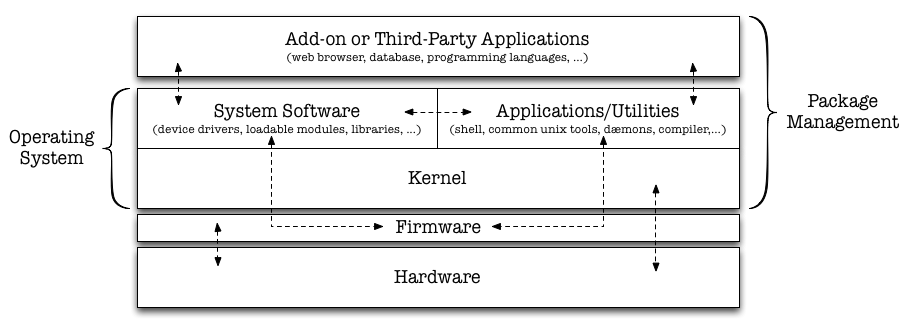
\includegraphics[scale=0.8]{pics/types-of-software.eps}
\end{center}
\vfill

\subsection{Base OS Installation}
General steps:
\begin{itemize}
	\item boot from boot media (CD, network, ...)
	\item identify root device
	\item optionally identify additional devices
	\item create partition table / disklabel
	\item create filesystem(s)
	\item install MBR, bootblocks etc.
	\item install / copy / extract OS
	\item optionally add application software
	\item perform basic system configuration
	\item reboot
\end{itemize}

\subsection{OS Installation}
\small
\begin{verbatim}
# fdisk -f -u 0 -s 169/63/4194241 /dev/rwd0d
# fdisk -f -c /usr/mdec/mbr /dev/rwd0d
# fdisk -f -a -0 /dev/rwd0d
# disklabel -e -I wd0
[...]
4 partitions:
#      size   offset fstype [fsize bsize cpg/sgs]
a:  4194241       63 4.2BSD    0     0      0 # (Cyl.      0*- 4161*)
c:  4194241       63 4.2BSD    0     0      0 # (Cyl.      0*- 4161*)
d:  4194304        0 unused    0     0      0 # (Cyl.      0 - 4161*)
# /sbin/newfs -O 2 /dev/rwd0a
/dev/rwd0a: 2048.0MB (4194240 sectors) block size 16384,
        fragment size 2048 using 12 cylinder groups of
        170.67MB, 10923 blks, 21504 inodes.
super-block backups (for fsck_ffs -b #) at:
32, 349568, 699104, 1048640, 1398176, 1747712, 2097248, 2446784,
....................................................................
# mount -o async /dev/wd0a /mnt
# for pkg in base comp etc games man misc modules text kern-GENERIC; do
tar zxpf /i386/binary/sets/${pkg}.tgz -C /mnt
done
# cp /mnt/usr/mdec/boot /mnt/boot
# /usr/sbin/installboot -v -o timeout=5 /dev/rwd0a \
        /mnt/usr/mdec/bootxx_ffsv2
File system:       /dev/rwd0a
Primary bootstrap: /usr/mdec/bootxx_ffsv2
Boot options:      timeout 5, flags 0, speed 9600, ioaddr 0, console pc
# cd /mnt/dev && ./MAKEDEV all
# shutdown -r now
\end{verbatim}
\Normalsize

\newpage
\vspace*{\fill}
\begin{center}
    \Hugesize
        Lecture 04 \\ [1em]
    \hspace*{5mm}
    \blueline\\
    \hspace*{5mm}\\
	Multiuser Fundamentals, Ethics
\end{center}
\vspace*{\fill}

\subsection{Implications of a Multi-User System}
\begin{itemize}
	\item users may want to keep files private
	\item users may want to share files
	\item users may (try to gain) access to files they shouldn't have access to
	\item users may (want to) do things that affect other users
	\item different users may require different privileges
\end{itemize}

\subsection{Ethics}
The LISA Code of Ethics:
\\

\newcolumntype{S}{>{\centering\arraybackslash} m{.4\linewidth} }
\begin{tabular}{ p{10cm} S }
\begin{itemize}
	\item Professionalism
	\item Personal Integrity
	\item Privacy
	\item Laws and Policies
	\item System Integrity
	\item Education
	\item Social Responsibility
	\item Ethical Responsibility
\end{itemize}
& \multirow{20}{*}{
\includegraphics[scale=1.3]{pics/angel.eps}} \\
\end{tabular}

\subsection{SysAdmin realities}
\begin{itemize}
	\item you are in a {\em privileged} position
	\item you {\em are} a target
	\item you are {\em obligated} to act in your users' interest
	\item you {\em will} face tough choices
	\item there is {\em no rulebook} to help you decide
	\item you {\em can} make a difference
\end{itemize}

\begin{center}
	
\includegraphics[scale=0.25]{pics/thumbsup-borat.eps}
\end{center}

\newpage
\vspace*{\fill}
\begin{center}
    \Hugesize
        Lecture 05 \\ [1em]
    \hspace*{5mm}
    \blueline\\
    \hspace*{5mm}\\
	Automating Administrative Tasks
\end{center}
\vspace*{\fill}

\subsection{Tools}
\vspace*{\fill}
\begin{center}
	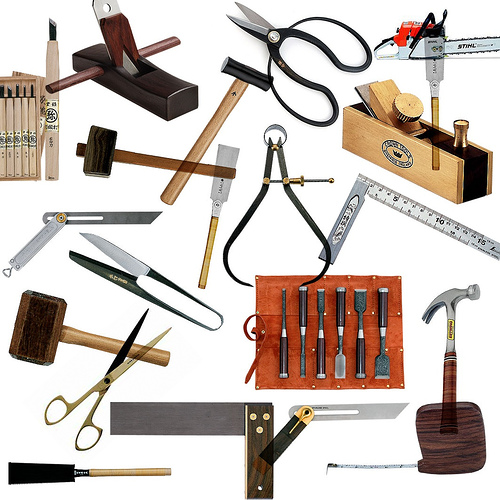
\includegraphics[scale=1.4]{pics/tools.eps}
\end{center}
\vspace*{\fill}

\subsection{Unix Philosophy}
\\
\Huge
\begin{center}
	Write programs that do one thing and do it well.\\
	\vspace{.5in}
	Write programs to work together. \\
	\vspace{.5in}
	Write programs to handle text streams, because that is a universal interface.
\end{center}
\Normalsize

\subsection{Know your languages / eco-system}
Some advice transcends language: \\

\small
\begin{verbatim}
$ echo import this | python
The Zen of Python, by Tim Peters

Beautiful is better than ugly.
Explicit is better than implicit.
Simple is better than complex.
Complex is better than complicated.
Flat is better than nested.
Sparse is better than dense.
Readability counts.
Special cases aren't special enough to break the rules.
Although practicality beats purity.
Errors should never pass silently.
Unless explicitly silenced.
In the face of ambiguity, refuse the temptation to guess.
There should be one-- and preferably only one --obvious way to do it.
Although that way may not be obvious at first unless you're Dutch.
Now is better than never.
Although never is often better than *right* now.
If the implementation is hard to explain, it's a bad idea.
If the implementation is easy to explain, it may be a good idea.
Namespaces are one honking great idea -- let's do more of those!
\end{verbatim}
\Normalsize

\subsection{Learn to write a detailed bug report}
Pre-requisite: Do your homework. \\

Required:
\begin{itemize}
	\item Description Of Problem
	\item Steps To Reproduce
	\item Expected Results
	\item Actual Results
\end{itemize}
\vspace{.125in}

Optional / recommended:
\begin{itemize}
	\item Screenshots / {\em exact} copy of terminal I/O ({\tt script(1)})
	\item Suggested Remediation
	\item Code Patch
\end{itemize}

\newpage
\vspace*{\fill}
\begin{center}
    \Hugesize
        Lecture 06 \\ [1em]
    \hspace*{5mm}
    \blueline\\
    \hspace*{5mm}\\
	Networking
\end{center}
\vspace*{\fill}

\subsection{Subnets}
\begin{verbatim}
$ ipcalc -n 155.246.89.22/24
Address:   155.246.89.22        10011011.11110110.01011001. 00010110
Netmask:   255.255.255.0 = 24   11111111.11111111.11111111. 00000000
Wildcard:  0.0.0.255            00000000.00000000.00000000. 11111111
=>
Network:   155.246.89.0/24      10011011.11110110.01011001. 00000000
HostMin:   155.246.89.1         10011011.11110110.01011001. 00000001
HostMax:   155.246.89.254       10011011.11110110.01011001. 11111110
Broadcast: 155.246.89.255       10011011.11110110.01011001. 11111111
Hosts/Net: 254                   Class B
\end{verbatim}
\vspace{.5in}
Try also: \verb+sipcalc -a 155.246.89.22/16+

\subsection{IPv6 Subnets}
\begin{verbatim}
$ sipcalc 2001:470:30:84:e276:63ff:fe72:3900/64
-[ipv6 : 2001:470:30:84:e276:63ff:fe72:3900/64] - 0

[IPV6 INFO]
Expanded Address        - 2001:0470:0030:0084:e276:63ff:fe72:3900
Compressed address      - 2001:470:30:84:e276:63ff:fe72:3900
Subnet prefix (masked)  - 2001:470:30:84:0:0:0:0/64
Address ID (masked)     - 0:0:0:0:e276:63ff:fe72:3900/64
Prefix address          - ffff:ffff:ffff:ffff:0:0:0:0
Prefix length           - 64
Address type            - Aggregatable Global Unicast Addresses
Network range           - 2001:0470:0030:0084:0000:0000:0000:0000 -
                          2001:0470:0030:0084:ffff:ffff:ffff:ffff

\end{verbatim}


\subsection{Mommy, where do IP addresses come from?}
\vspace*{\fill}
\begin{center}
	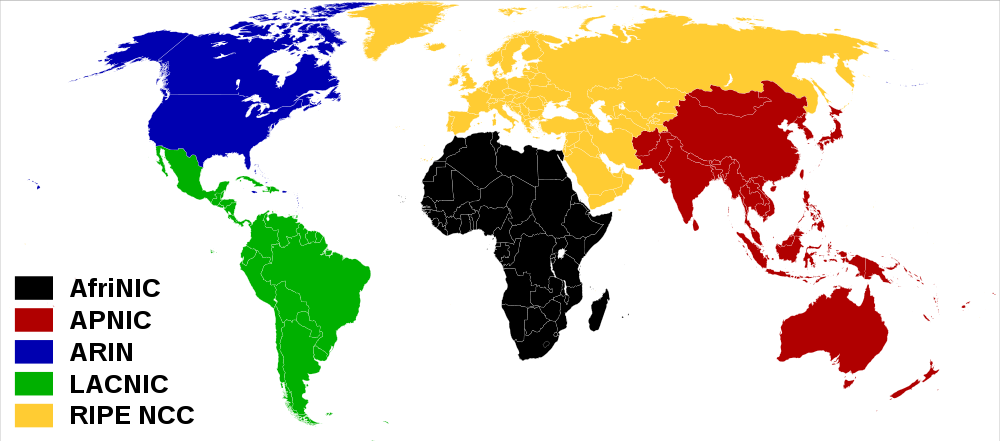
\includegraphics[scale=0.5]{pics/rirs.eps} \\
	\vspace{.5in}
	Regional Internet Registries (RIR) manage the allocation and
registration of Internet number resources within a region of the world.
\end{center}
\vspace*{\fill}

\subsection{Networking}
Stringing cables across the oceans' floors since 1866!
\vspace*{\fill}
\begin{center}
	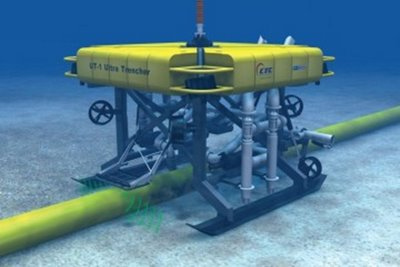
\includegraphics[scale=1.0]{pics/internet-undersea-cable.eps} \\
	\verb+http://www.submarinecablemap.com/+ \\
	\verb+http://is.gd/CjanOu+
\end{center}
\vspace*{\fill}

\subsection{A simple example}
\\
\Hugesize
\begin{center}
\begin{verbatim}
$ strace -f telnet www.google.com 80 2>strace.out
Trying 173.194.73.99...
Connected to www.google.com.
Escape character is '^]'.
GET / HTTP/1.0

[...]
\end{verbatim}
\end{center}
\Normalsize
\vspace*{\fill}

\subsection{...open a few files...}
\begin{verbatim}
execve("/usr/bin/telnet", ["telnet", "www.google.com", "80"], [/* 29 vars */]) = 0
[...]
open("/etc/nsswitch.conf", O_RDONLY)    = 3
fstat(3, {st_mode=S_IFREG|0644, st_size=286, ...}) = 0
mmap(NULL, 4096, PROT_READ|PROT_WRITE, MAP_PRIVATE|MAP_ANONYMOUS, -1, 0) = [...]
read(3, "passwd: files ldap\ngroup: files "..., 4096) = 286
[...]
open("/etc/hosts", O_RDONLY|O_CLOEXEC)  = 3
fcntl(3, F_GETFD)                       = 0x1 (flags FD_CLOEXEC)
fstat(3, {st_mode=S_IFREG|0644, st_size=277, ...}) = 0
mmap(NULL, 4096, PROT_READ|PROT_WRITE, MAP_PRIVATE|MAP_ANONYMOUS, -1, 0) = [...]
read(3, "127.0.0.1    localhost\n\n# The fo"..., 4096) = 277
[...]
stat("/etc/resolv.conf", {st_mode=S_IFREG|0644, st_size=205, ...}) = 0
open("/etc/resolv.conf", O_RDONLY)      = 3
fstat(3, {st_mode=S_IFREG|0644, st_size=205, ...}) = 0
read(3, "nameserver 155.246.1.20\nnameserv"..., 4096) = 205
\end{verbatim}

\subsection{... query a DNS server ...}
\begin{verbatim}
[...]
socket(PF_INET, SOCK_DGRAM|SOCK_NONBLOCK, IPPROTO_IP) = 3
connect(3, {sa_family=AF_INET, sin_port=htons(53),
        sin_addr=inet_addr("155.246.1.20")}, 16) = 0
gettimeofday({1330805293, 202924}, NULL) = 0
sendto(3, "\364\333\1\0\0\1\0\0\0\0\0\0\3www\6google\3com\0\0\1\0\1", 32,
        MSG_NOSIGNAL, NULL, 0) = 32
poll([{fd=3, events=POLLIN}], 1, 5000)  = 1 ([{fd=3, revents=POLLIN}])
ioctl(3, FIONREAD, [504])               = 0
recvfrom(3, "\364\333\201\200\0\1\0\6\0\r\0\10\3www\6google\3com\0\0\1\0\1"...,
        1024, 0, {sa_family=AF_INET, sin_port=htons(53),
        sin_addr=inet_addr("155.246.1.20")}, [16]) = 504
close(3)                                = 0
[...]
\end{verbatim}

\subsection{...communicate with the remote host...}
\begin{verbatim}
[...]
write(1, "Trying 173.194.73.104...\n", 25) = 25
close(4294967295)                       = -1 EBADF (Bad file descriptor)
socket(PF_INET, SOCK_STREAM, IPPROTO_IP) = 3
setsockopt(3, SOL_IP, IP_TOS, [16], 4)  = 0
connect(3, {sa_family=AF_INET, sin_port=htons(80),
        sin_addr=inet_addr("173.194.73.104")},16) = 0
[...]
read(0, "GET / HTTP/1.0\n", 8191)       = 15
select(4, [0 3], [3], [3], {0, 0})      = 1 (out [3], left {0, 0})
sendto(3, "GET / HTTP/1.0\r\n", 16, 0, NULL, 0) = 16
[...]
recvfrom(3, "HTTP/1.0 200 OK\r\nDate: Sat, 02 M"..., 8191, 0, NULL, NULL) = 5520
select(4, [0 3], [1], [3], {0, 0})      = 2 (in [3], out [1], left {0, 0})
write(1, "HTTP/1.0 200 OK\nDate: Sat, 02 Ma"..., 5508) = 5508
recvfrom(3, "", 6035, 0, NULL, NULL)    = 0
[...]
\end{verbatim}

\subsection{TCP/IP Basics: ARP}
\vspace*{\fill}
\begin{center}
	\includegraphics[scale=0.8]{pics/3computers-arp.eps}
\end{center}
\vspace*{\fill}

\subsection{TCP/IP Basics: ICMP: Ping}
\vspace*{\fill}
\begin{center}
	\includegraphics[scale=0.8]{pics/3computers-ping.eps}
\end{center}
\vspace*{\fill}


\subsection{TCP/IP Basics: ICMP: Traceroute}
\vspace*{\fill}
\begin{center}
	\includegraphics[scale=0.8]{pics/traceroute4.eps}
\end{center}
\vspace*{\fill}

\subsection{Networking}
\vspace*{\fill}
\begin{center}
	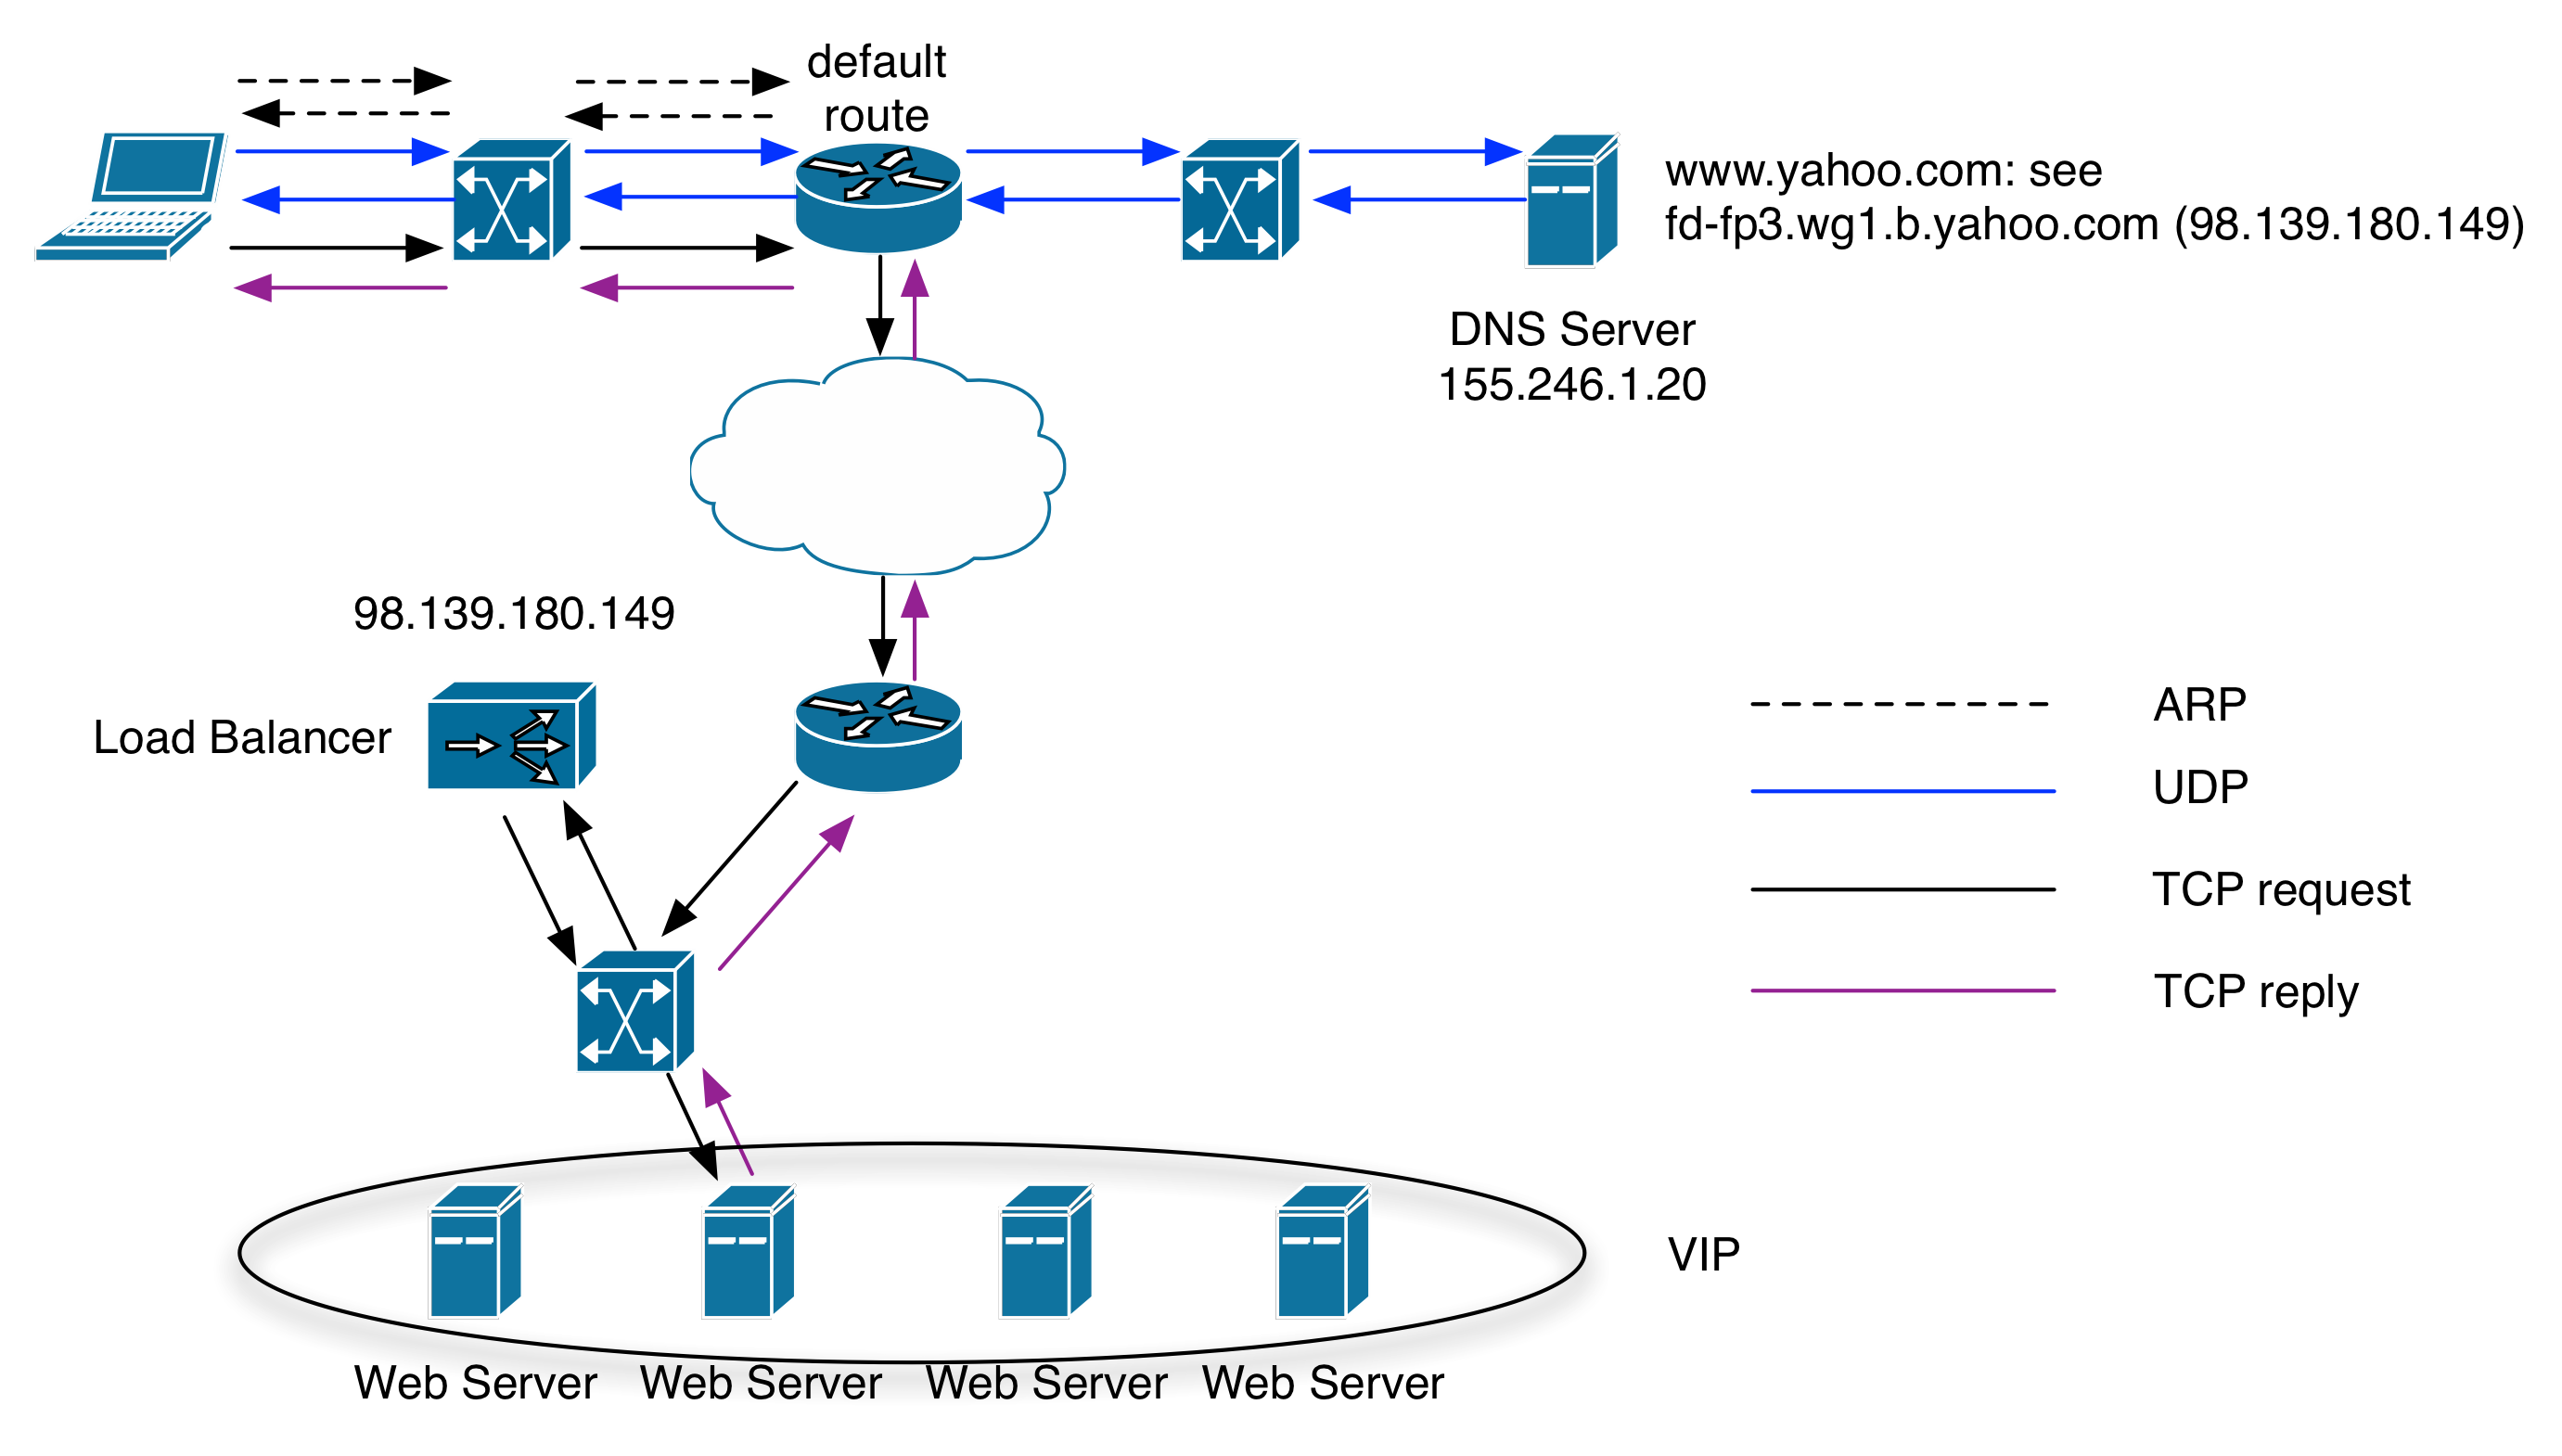
\includegraphics[scale=0.8]{pics/dsr.eps} \\
\end{center}
\vspace*{\fill}

\subsection{TCP/IP Basics: Putting it all together}
\vspace*{\fill}
\begin{center}
	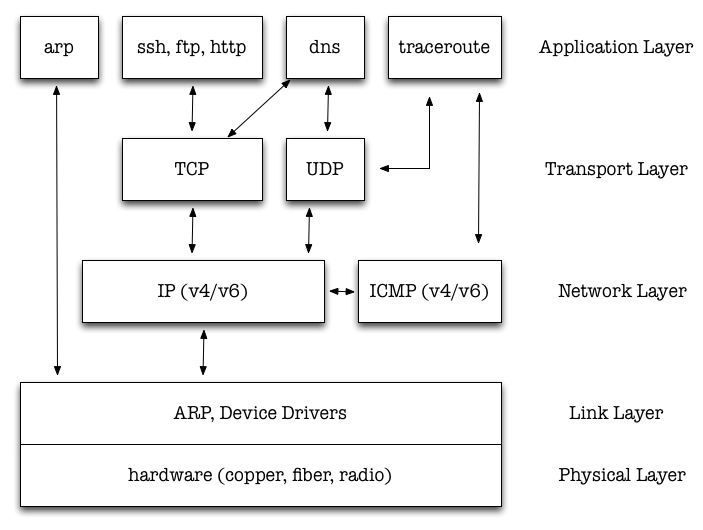
\includegraphics[scale=0.6]{pics/tcpip-stack.eps}
\end{center}
\vspace*{\fill}

\newpage
\vspace*{\fill}
\begin{center}
    \Hugesize
        Lecture 07 \\ [1em]
    \hspace*{5mm}
    \blueline\\
    \hspace*{5mm}\\
	DNS; Backup and Disaster Recovery
\end{center}
\vspace*{\fill}

\subsection{The New Phonebook is here!}
\vspace*{\fill}
\begin{center}
	\verb+http://is.gd/XXp2sC+ \\
	\addvspace{.5in}
	\verb+wget -q -O - http://is.gd/XXp2sC | grep -c "^HOST"+
\end{center}
\vspace*{\fill}

\subsection{DNS: A hierarchical system}
\vspace*{\fill}
\begin{center}
	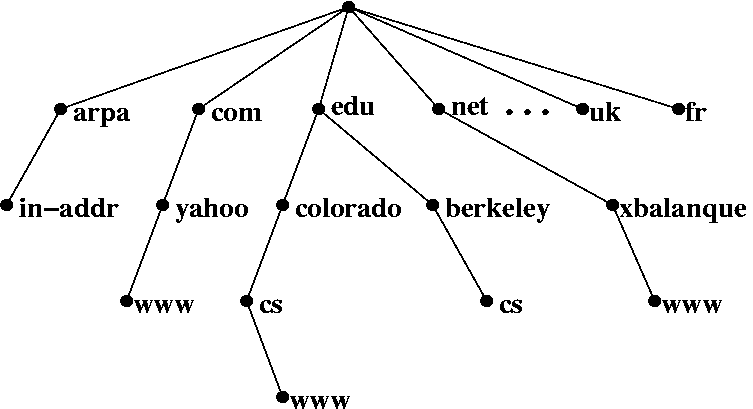
\includegraphics[scale=0.75]{pics/hierarchical-dns.eps}
\end{center}
\vspace*{\fill}

\subsection{Hostname resolution}
\vspace*{\fill}
\begin{center}
	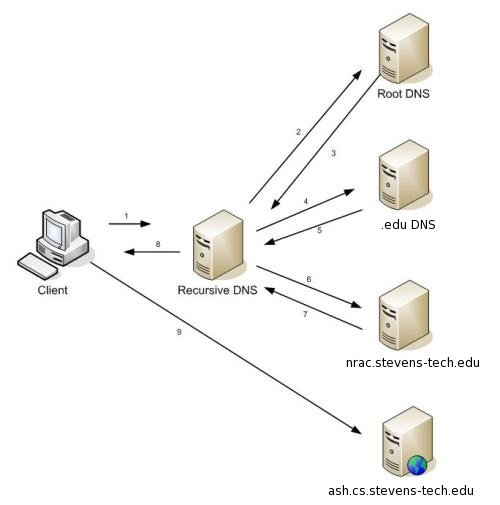
\includegraphics[scale=0.9]{pics/resolution.eps}
\end{center}
\vspace*{\fill}

\subsection{DNS: A distributed database}
\vspace*{\fill}
\begin{center}
	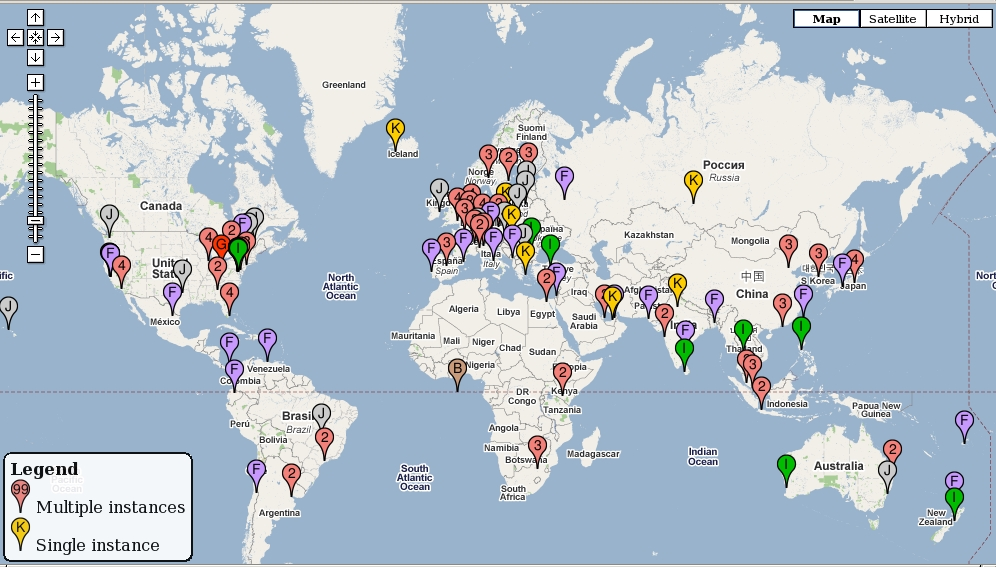
\includegraphics[scale=0.5]{pics/root-servers.eps}
\end{center}
\vspace*{\fill}

\subsection{Creative uses of DNS Resource Records}
\begin{itemize}
	\item identifying sources of SPAM
	\item find out if the internet is on fire: \\
		\verb|dig +short txt istheinternetonfire.com|
	\item find ASN numbers by IP addresses: \\
		\verb|dig +short 159.89.246.155.origin.asn.cymru.com TXT|
	\item check a resolver's source port randomization (to help
		mitigate DNS Cache Poisoning attacks): \\
		\verb|dig +short porttest.dns-oarc.net TXT|
	\item using DNS to publish SSH key fingerprints (RFC4255,
ssh\_config(5) \verb+VerifyHostKeyDNS+; for best results combine with DNSSEC): \\
		\verb|dig +short ftp.netbsd.org SSHFP|
		\begin{verbatim}
ssh -o "VerifyHostKeyDNS yes" ftp.netbsd.org
[...]
Matching host key fingerprint found in DNS.
Are you sure you want to continue connecting (yes/no)?
\end{verbatim}
\end{itemize}

\newpage
\vspace*{\fill}
\begin{center}
    \Hugesize
        Presentation \\ [1em]
    \hspace*{5mm}
    \blueline\\
    \hspace*{5mm}\\
	Bipin Pandey
\end{center}
\vspace*{\fill}

\subsection{Backups and Restore Basics}
When do we need backups?
\begin{itemize}
	\item disaster recovery: off-site storage of sensitive data
	\item long-term storage requirements
	\item recover from data loss due to
		\begin{itemize}
			\item equipment failure
			\item bozotic users
			\item natural disaster
			\item security breach
			\item software bugs
		\end{itemize}
\end{itemize}
\addvspace{.5in}
Think of your backups as {\em insurance}:  you invest and pay for it, hoping
you will never need it.

\subsection{Filesystem backup}
Example: WAFL (Write Anywhere File Layout)
\vspace*{\fill}
\begin{center}
	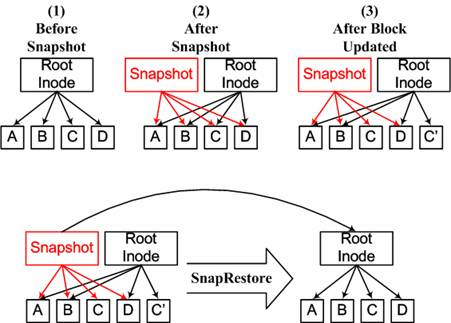
\includegraphics[scale=1.0]{pics/wafl.eps}
\end{center}
\vspace*{\fill}

\newpage
\vspace*{\fill}
\begin{center}
    \Hugesize
        Lecture 08 \\ [1em]
    \hspace*{5mm}
    \blueline\\
    \hspace*{5mm}\\
	SMTP, HTTP
\end{center}
\vspace*{\fill}

\subsection{Sending...}
\begin{verbatim}
# tcpdump -i xennet0 -w /tmp/t.out port not 22 2>/dev/null &
# mail -s "CS615 - SMTP Exercise" jschauma@stevens.edu -f jschauma@stevens.edu
Hello,

SMTP is simple.

-Jan
.
EOT
# fg
tcpdump -i xennet0 -w /tmp/t.out port not 22 2>/dev/null
^C
\end{verbatim}

\subsection{Sending...}
\begin{verbatim}
# tail -5 /var/log/maillog
Apr  4 15:42:33 ip-10-235-167-232 postfix/pickup[848]: 2A17275438:
        uid=0 from=<jschauma@stevens.edu>
Apr  4 15:42:33 ip-10-235-167-232 postfix/cleanup[765]: 2A17275438:
        message-id=<20160404154233.2A17275438@ip-10-235-167-232.ec2.internal>
Apr  4 15:42:33 ip-10-235-167-232 postfix/qmgr[876]: 2A17275438:
        from=<jschauma@stevens.edu>, size=380, nrcpt=1 (queue active)
Apr  4 15:42:33 ip-10-235-167-232 postfix/smtp[1124]: 2A17275438:
        to=<jschauma@stevens.edu>, relay=spamfilter01.stevens.edu[155.246.14.37]:25,
        delay=0.62, delays=0.04/0.01/0.03/0.54, dsn=2.0.0,
        status=sent (250 Ok: queued as 688CD6F4001)
Apr  4 15:42:33 ip-10-235-167-232 postfix/qmgr[876]: 2A17275438: removed
\end{verbatim}

\subsection{Sending...}
\begin{verbatim}
# tcpdump -t -r /tmp/t.out port 53
IP 10.235.167.232.65498 > 172.16.0.23.domain: 61195+ MX? stevens.edu. (29)
IP 172.16.0.23.domain > 10.235.167.232.65498: 61195 2/0/0
        MX spamfilter01.stevens.edu. 10,
        MX spamfilter02.stevens.edu. 20 (87)
IP 10.235.167.232.65497 > 172.16.0.23.domain: 1949+
        A? spamfilter01.stevens.edu. (42)
IP 172.16.0.23.domain > 10.235.167.232.65497: 1949 1/0/0 A 155.246.14.37 (58)
IP 10.235.167.232.65496 > 172.16.0.23.domain: 39922+
        AAAA? spamfilter01.stevens.edu. (42)
IP 172.16.0.23.domain > 10.235.167.232.65496: 39922 0/1/0 (113)
IP 10.235.167.232.65495 > 172.16.0.23.domain: 26844+
        A? spamfilter02.stevens.edu. (42)
IP 172.16.0.23.domain > 10.235.167.232.65495: 26844 1/0/0 A 155.246.248.24 (58)
IP 10.235.167.232.65494 > 172.16.0.23.domain: 1439+
        AAAA? spamfilter02.stevens.edu. (42)
IP 172.16.0.23.domain > 10.235.167.232.65494: 1439 0/1/0 (113)
\end{verbatim}

\subsection{Sending...}
\begin{Verbatim}
$ telnet 155.246.14.37 25
Trying 155.246.14.37...
Connected to spamfilter01.stevens.edu.
Escape character is '^]'.
\textbf{220 spamfilter01.stevens.edu ESMTP (fe32969a29a5f461e53bf93b18c8fdb5)}
EHLO ip-10-235-167-232.ec2.internal
\textbf{250-spamfilter01.stevens.edu Hello ec2-54-205-68-41.compute-1.amazonaws.com [54.205.68.41],}
\textbf{        pleased to meet you}
\textbf{250-SIZE 50000000}
\textbf{250-PIPELINING}
\textbf{250-8BITMIME}
\textbf{250 HELP}
MAIL FROM:<jschauma@stevens.edu> SIZE=380
\textbf{250 Sender <jschauma@stevens.edu> OK}
RCPT TO:<jschauma@stevens.edu>
\textbf{250 Recipient <jschauma@stevens.edu> OK}
\end{Verbatim}

\subsection{Sending...}
\begin{Verbatim}
DATA
\textbf{354 Start mail input; end with <CRLF>.<CRLF>}
Received: by ip-10-235-167-232.ec2.internal (Postfix, from userid 0)
        id 2A17275438; Mon,  4 Apr 2016 15:42:33 +0000 (UTC)
To: jschauma@stevens.edu
Subject: CS615 - SMTP Exercise
Message-Id: <20160404154233.2A17275438@ip-10-235-167-232.ec2.internal>
Date: Mon,  4 Apr 2016 15:42:33 +0000 (UTC)
From: jschauma@stevens.edu (Charlie Root)

Hello,

SMTP is simple.

-Jan
.
\textbf{250 Ok: queued as 6A9C76F4004}
\end{Verbatim}



\subsection{Receiving...}
\begin{verbatim}
Date: Mon, 4 Apr 2016 15:42:33 +0000
From: Jan Schaumann <jschauma@stevens.edu>
To: Jan Schaumann <jschauma@stevens.edu>
Subject: CS615 - SMTP Exercise

Hello,

SMTP is simple.

-Jan
\end{verbatim}

\subsection{Receiving...}
\smallish
\begin{verbatim}
From jschauma@stevens.edu  Mon Apr  4 11:42:35 2016
Received: by panix.netmeister.org (Postfix, from userid 1004)
        id 6B0F56513D; Mon,  4 Apr 2016 11:42:35 -0400 (EDT)
Received: from nexus.stevens.edu (nexus.stevens.edu [155.246.14.12])
        by panix.netmeister.org (Postfix) with ESMTP id 2AD596513B
Received: from exchng02.campus.stevens-tech.edu (exchng02.campus.stevens-tech.edu [155.246.14.23])
        by nexus.stevens.edu (Postfix) with ESMTPS id 11E3817F825
Received: from exchng04.campus.stevens-tech.edu (2002:9bf6:f826::9bf6:f826) by
        exchng02.campus.stevens-tech.edu (2002:9bf6:e17::9bf6:e17) with Microsoft
        SMTP Server (TLS) id 15.0.1104.5; Mon, 4 Apr 2016 11:42:34 -0400
Received: from exchng03.campus.stevens-tech.edu (155.246.248.36) by
        exchng04.campus.stevens-tech.edu (155.246.248.39) with Microsoft SMTP Server
        (TLS) id 15.0.1104.5; Mon, 4 Apr 2016 11:42:34 -0400
Received: from exchng03.campus.stevens-tech.edu ([::1]) by
        exchng03.campus.stevens-tech.edu ([fe80::599a:f128:d1b3:4ce7%12]) with
        Microsoft SMTP Server id 15.00.1104.000; Mon, 4 Apr 2016 11:42:34 -0400
From: Jan Schaumann <jschauma@stevens.edu>
To: Jan Schaumann <jschauma@stevens.edu>
Subject: CS615 - SMTP Exercise
Date: Mon, 4 Apr 2016 15:42:33 +0000
Message-ID: <1b1399e9c44b494f99e9d0030f0fa74b@exchng03.campus.stevens-tech.edu>
x-barracuda-apparent-source-ip: 54.205.68.41
x-ms-exchange-parent-message-id: <20160404154233.2A17275438@ip-10-235-167-232.ec2.internal>
Resent-Message-Id: <20160404154235.11E3817F825@nexus.stevens.edu>
\end{verbatim}

\newpage
\vspace*{\fill}
\begin{center}
    \Hugesize
        Presentation \\ [1em]
    \hspace*{5mm}
    \blueline\\
    \hspace*{5mm}\\
	Avineshwar Pratap Singh
\end{center}
\vspace*{\fill}


\subsection{The Hypertext Transfer Protocol}
HTTP is a request/response protocol:
\begin{enumerate}
	\item client sends a request to the server
		\begin{itemize}
			\item request method
			\item URI
			\item protocol version
			\item request modifiers
			\item client information
		\end{itemize}
	\item server responds
		\begin{itemize}
			\item status line (including success or error code)
			\item server information
			\item entity metainformation
			\item content
		\end{itemize}
\end{enumerate}

\subsection{HTTP: A client request}
\begin{center}
	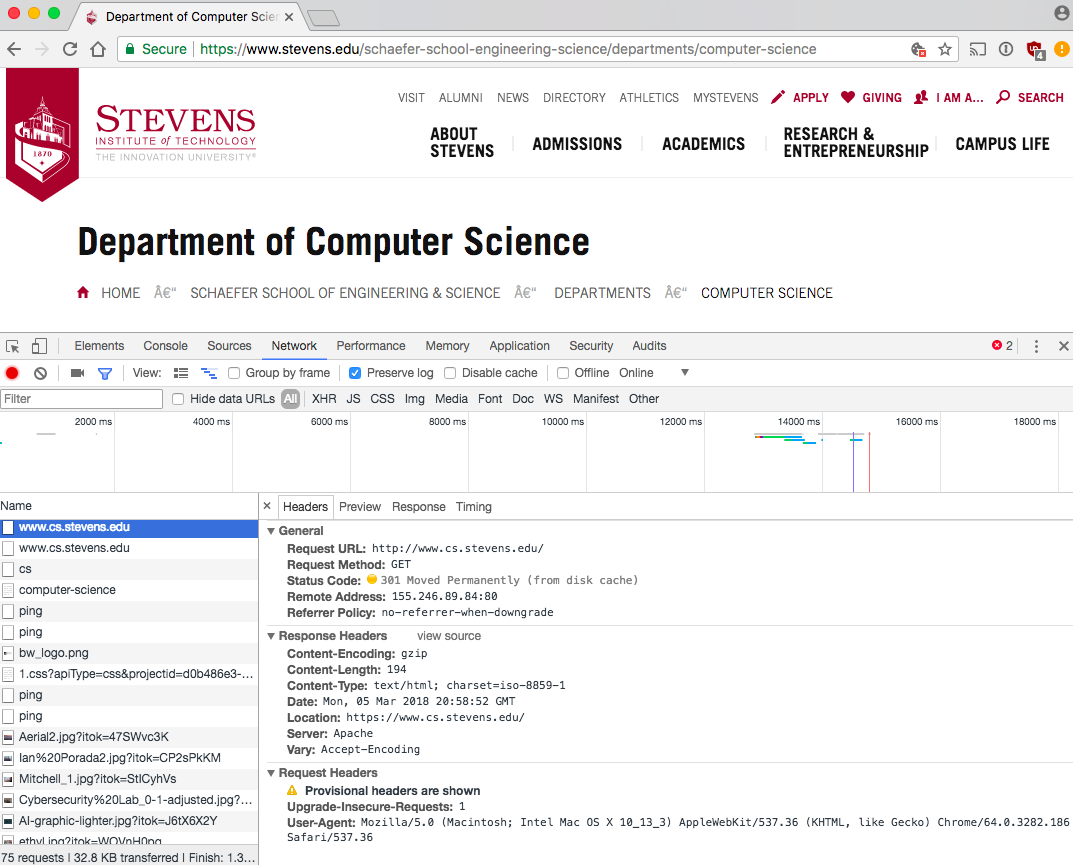
\includegraphics[scale=0.6]{pics/www.cs.stevens.edu.eps}
\end{center}

\subsection{HTTP overload}
Ways to mitigate HTTP overload:

\begin{itemize}
	\item DNS round-robin to many web servers
	\item load balancing
	\item web cache / accelerators (reverse proxies)
	\item content delivery networks
\end{itemize}

These solutions depend on the location within the network and the scale of
the environment.

\newpage
\vspace*{\fill}
\begin{center}
    \Hugesize
        Lecture 09 \\ [1em]
    \hspace*{5mm}
    \blueline\\
    \hspace*{5mm}\\
	HTTPS, Monitoring
\end{center}
\vspace*{\fill}

\subsection{TLS}
Transport Layer Security
\begin{itemize}
	\item set of cryptographic protocols
	\item operates on layer 6 of OSI stack (Presentation Layer)
	\item independent of HTTP
	\item RFC5246 (TLS 1.2)
\end{itemize}
\addvspace{.5in}
Two distinct security mechanisms:
\begin{enumerate}
	\item encryption of data in transit
	\item authentication of parties
\end{enumerate}

\subsection{TLS}
Protocol:
\begin{itemize}
	\item Client Hello, present list of supported cipher suites
	\item Server Hello, chosen cipher suite
	\item Server Certificate
	\item (Server Key Exchange Message), (Client Certificate Request), (Client Certificate)
	\item Client Key Exchange Message
	\item (Certificate Verify)
	\item (Client Change Cipher Spec), (Server Change Cipher Spec)
\end{itemize}

\subsection{TLS}
\begin{center}
	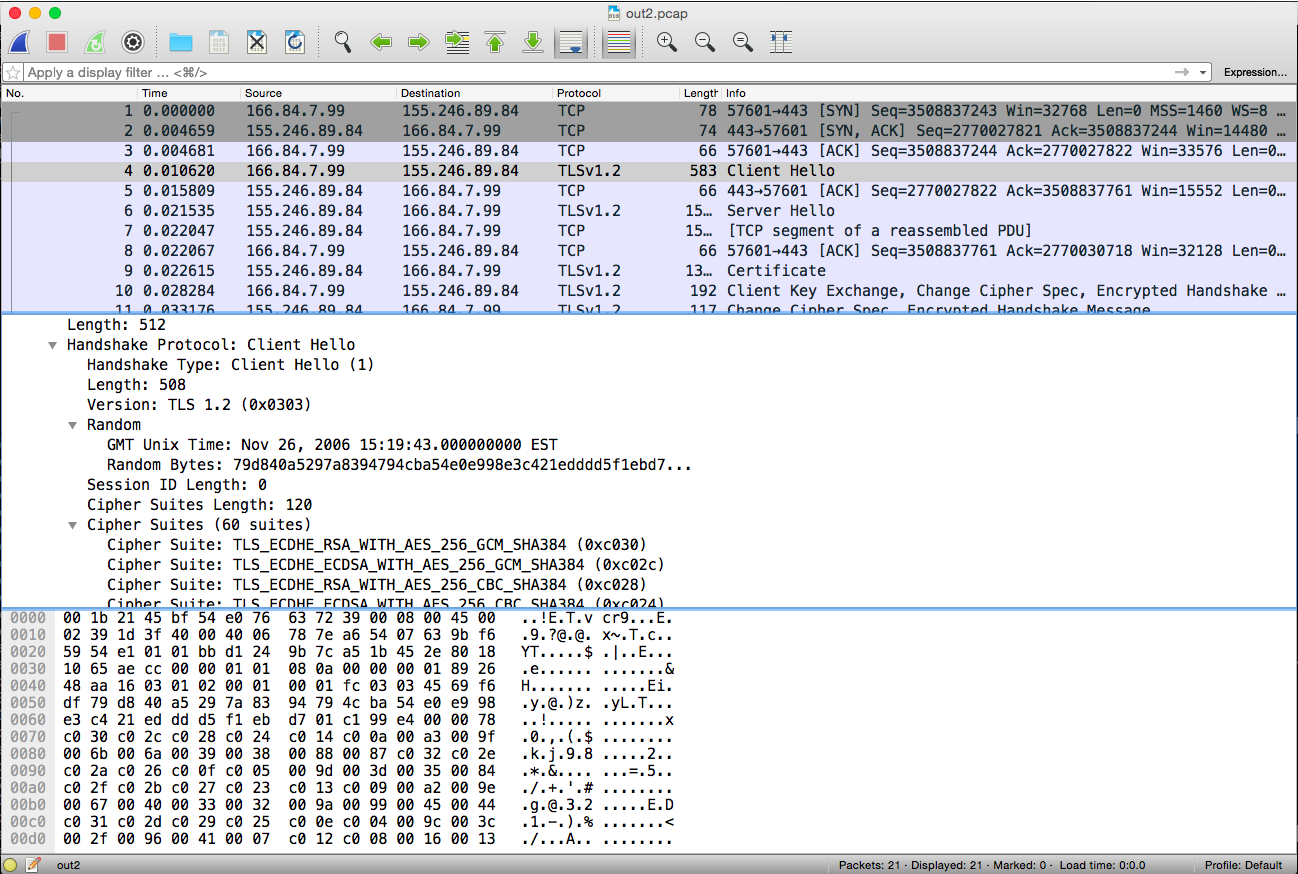
\includegraphics[scale=0.4]{pics/wireshark.eps}
\end{center}

\subsection{TLS}
\begin{verbatim}
$ openssl s_client -connect www.cs.stevens.edu:443
[...]
New, TLSv1/SSLv3, Cipher is DHE-RSA-AES256-SHA
Server public key is 2048 bit
Secure Renegotiation IS supported
Compression: NONE
Expansion: NONE
SSL-Session:
    Protocol  : TLSv1
    Cipher    : DHE-RSA-AES256-SHA
    Session-ID: 5F8A9B7A93EF87009EFCC17BBD68938C56EAACD9DF4C3643EF034D047C9F44C9
    Session-ID-ctx: 
    Master-Key: 20CBA1E477A8B573F29759045329EF7AA38C763C4C41606A46FBCC824C3F32F708789311E7B4275470E35CF09518FDCD
    Key-Arg   : None
    Start Time: 1460395966
    Timeout   : 300 (sec)
    Verify return code: 0 (ok)
\end{verbatim}

\subsection{TLS}
\begin{verbatim}
$ openssl s_client -connect www.cs.stevens.edu:443 | \
        openssl x509 -text -noout
[...]
        Signature Algorithm: sha1WithRSAEncryption
        Issuer: C=US, ST=Arizona, L=Scottsdale, O=GoDaddy.com, Inc., OU=http://certificates.godaddy.com/repository, CN=Go Daddy Secure Certification Authority/serialNumber=07969287
        Validity
            Not Before: Apr 22 13:14:11 2013 GMT
            Not After : Nov  8 15:26:38 2016 GMT
        Subject: OU=Domain Control Validated, CN=www.srcit.stevens.edu
        Subject Public Key Info:
            Public Key Algorithm: rsaEncryption
            RSA Public Key: (2048 bit)
[...]
            X509v3 Subject Alternative Name: 
                DNS:www.srcit.stevens.edu, DNS:srcit.stevens.edu, DNS:svn.srcit.stevens.edu,
                DNS:www.cs.stevens.edu, DNS:guinness.cs.stevens.edu, DNS:rcs.srcit.stevens.edu
\end{verbatim}

\subsection{Requesting a certificate}
\begin{center}
	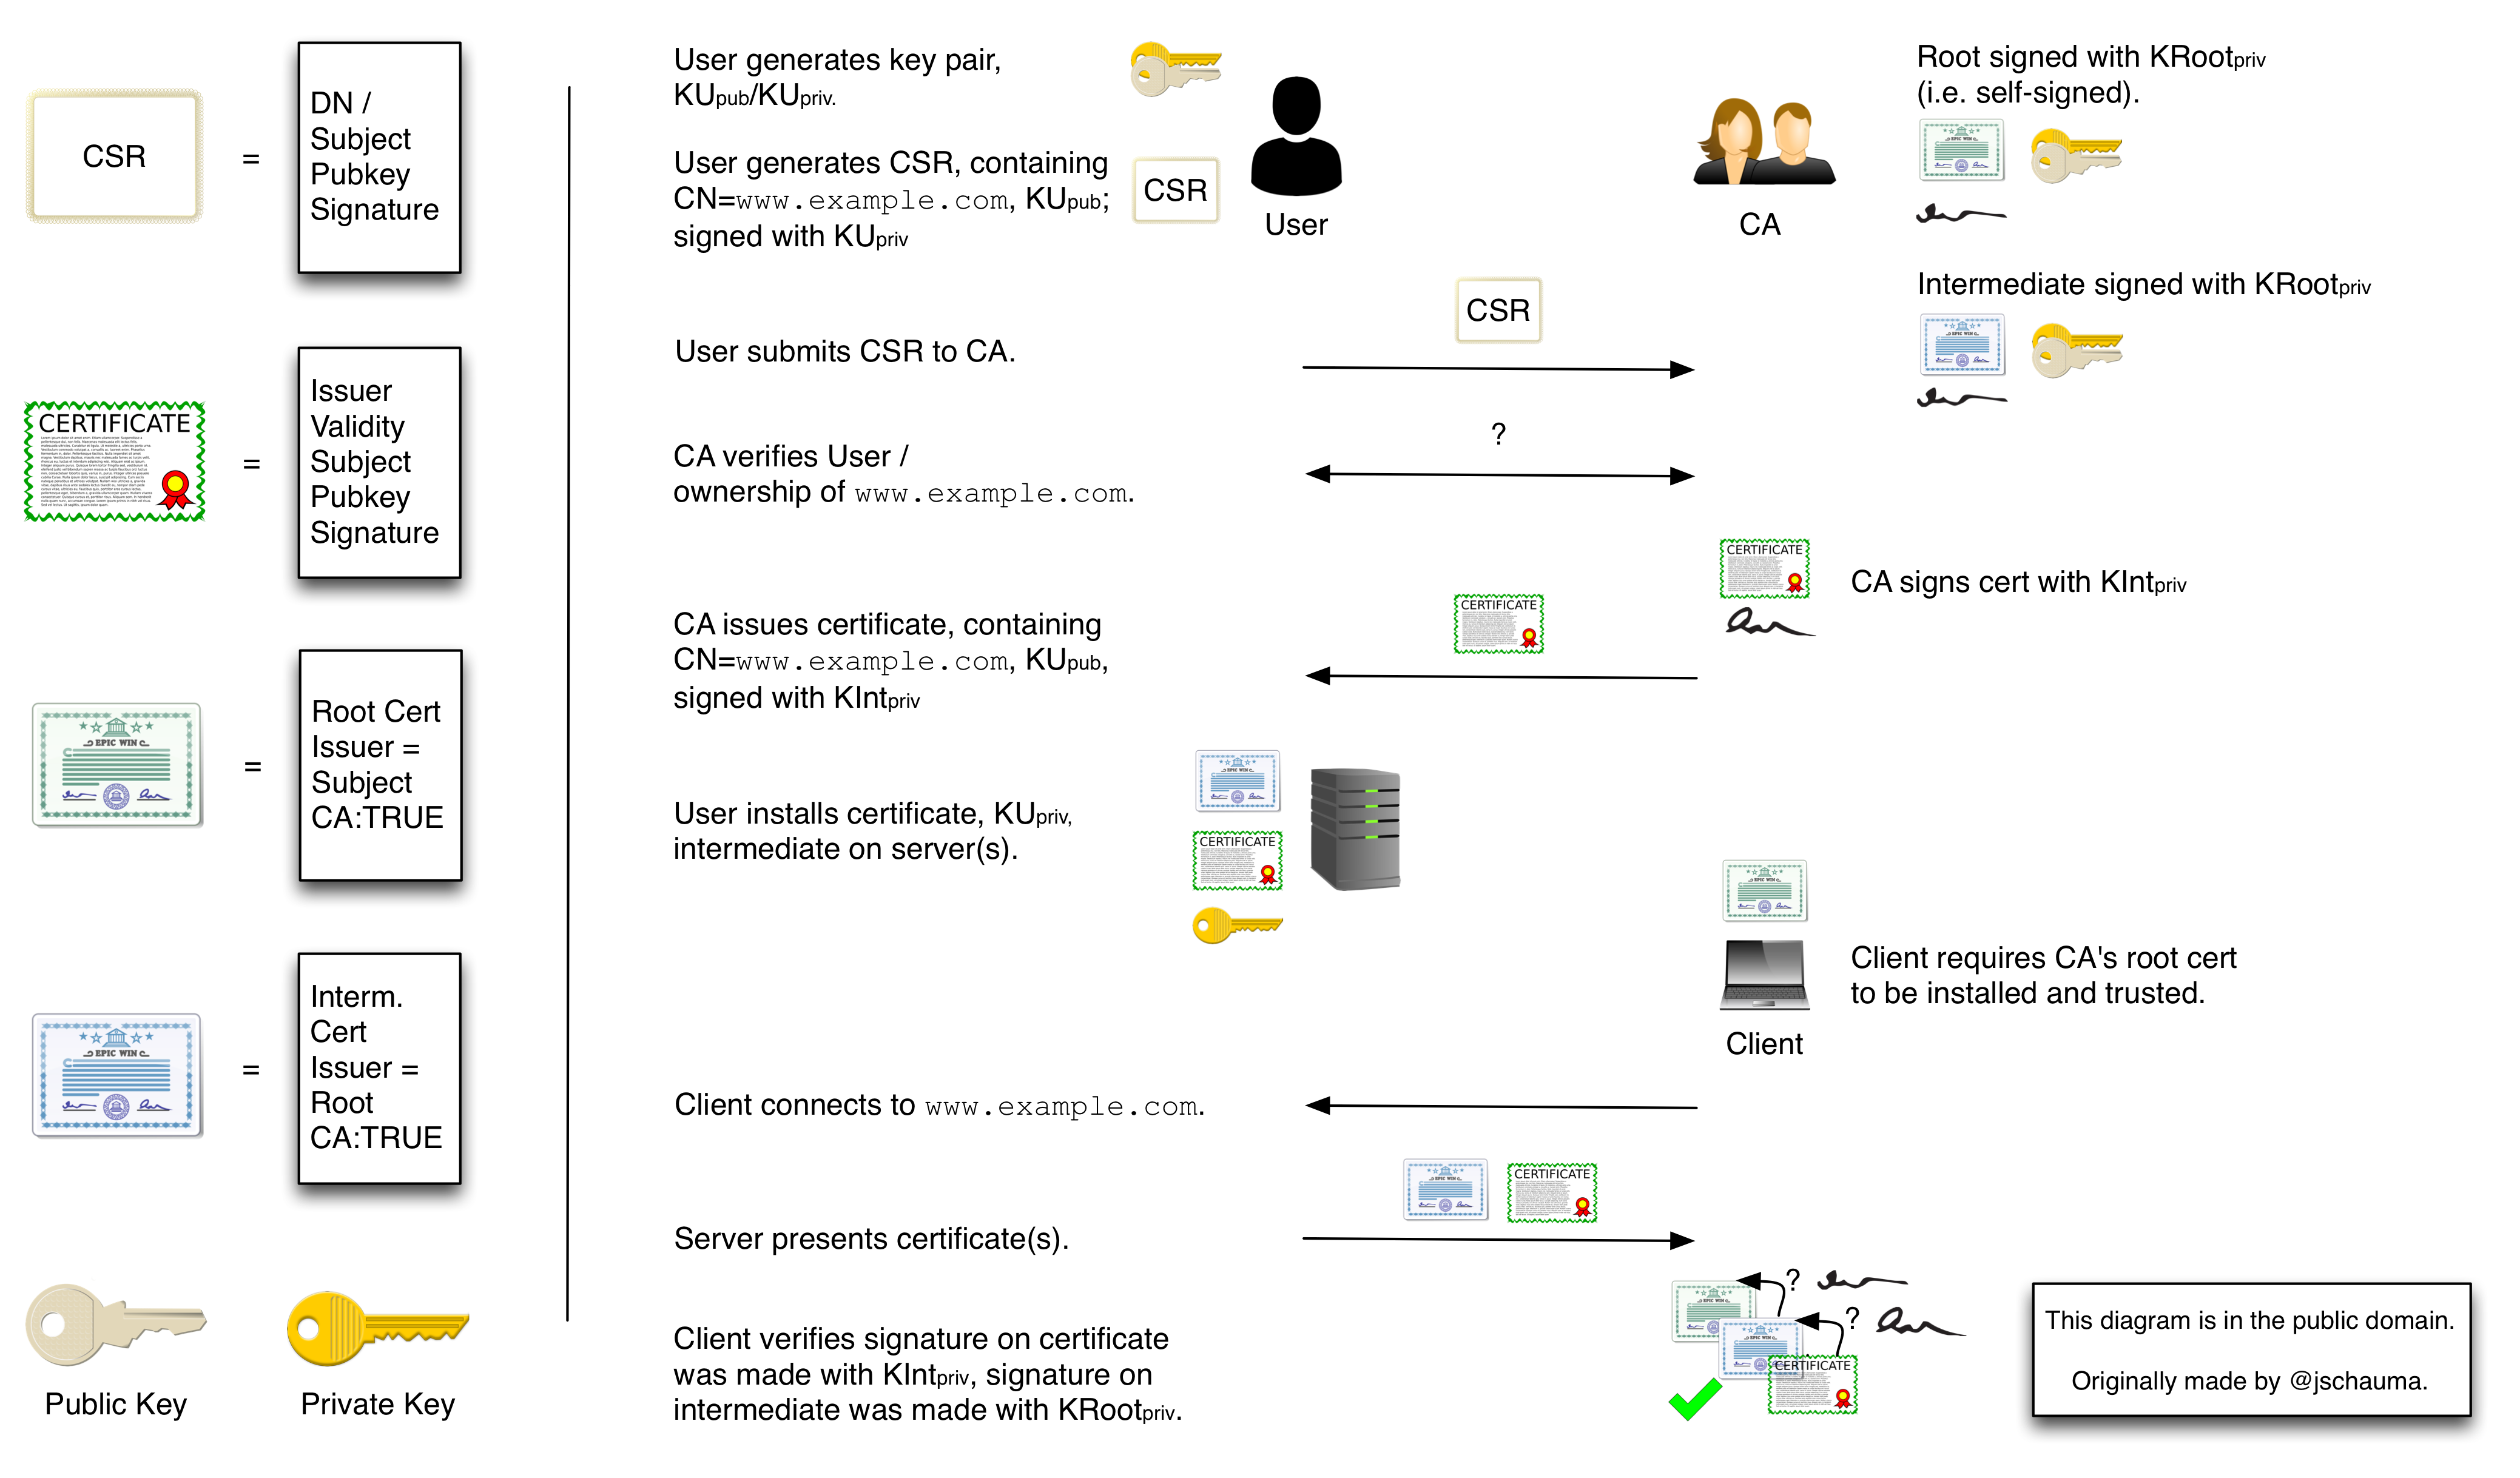
\includegraphics[scale=0.6]{pics/csr-process.eps}
\end{center}

\subsection{TLS Pitfalls}
Lack of universal HTTPS exposes users to significant
risks; many sites don't get the importance of
authentication for non-sensitive content. \\

In order to serve content, you need to have the
private key $ => $ privkey available at perimeter and
exposed, high-risk systems. \\

Rotation/renewal of keys requires routine processes,
which further expose the private key. \\

Control of a CA or a CA's key grants you near
universal powers. \\


\subsection{TLS Pitfalls}
Complex protocols, buggy implementations, intentional
weaknesses and backwards compatibility are just the
high level points.

\begin{itemize}
	\item SSLv2 obsoleted in 1996; 2016: DROWN attack
	\item SSLv3 obsoleted in 1999; 2014: POODLE attack
	\item BEAST, CRIME, BREACH, HEARTBLEED, GotoFail...
	\item obsolete and broken algorithms widely used (RC4, MD5, SHA1, ...)
\end{itemize}

\newpage
\vspace*{\fill}
\begin{center}
    \Hugesize
        Presentation \\ [1em]
    \hspace*{5mm}
    \blueline\\
    \hspace*{5mm}\\
	Smruthi Karinatte
\end{center}
\vspace*{\fill}

\subsection{Events}
\vspace*{\fill}
\Huge
\begin{center}
``Something's wrong.'' is just an {\em unexpected} or
{\em undesirable} event. \\
\vspace{.4in}
{\em Events} happen all the time. \\
\vspace{.4in}
Being able to identify {\em relevant} events allows
you to diagnose, predict and even prevent {\em
undesirable} events.
\end{center}
\Normalsize
\vspace*{\fill}

\subsection{Events and Metrics}
\vspace*{\fill}
\begin{verbatim}
$ dict event
  event
      n 1: something that happens at a given place and time
      2: a special set of circumstances; "in that event, the first
         possibility is excluded"; "it may rain in which case the
         picnic will be canceled" [syn: {event}, {case}]


$ dict metric
  metric
      3: a system of related measures that facilitates the
         quantification of some particular characteristic [syn:
         {system of measurement}, {metric}]

\end{verbatim}
\vspace*{\fill}

\subsection{Events and Metrics}
\begin{center}
	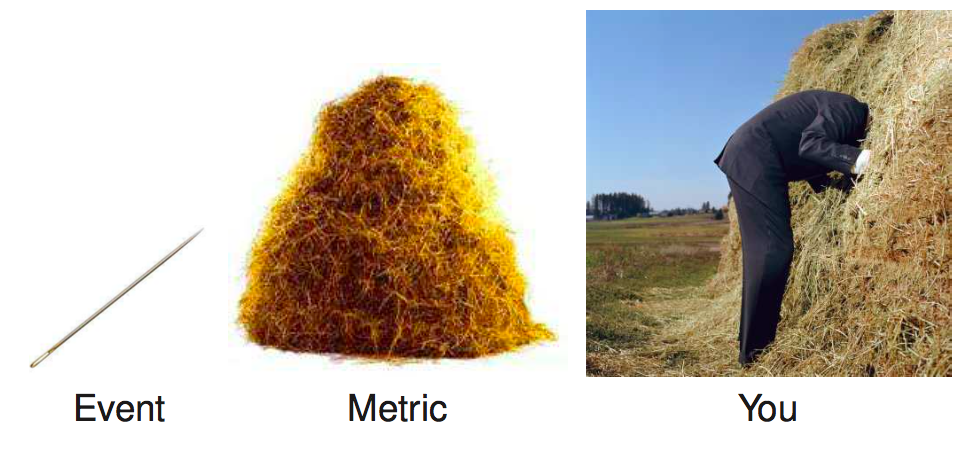
\includegraphics[scale=0.75]{pics/events-metrics.eps}
\end{center}

\subsection{Context}
{\em Context} lets you find {\em relevant} events in
your haystack of metrics.

\begin{center}
	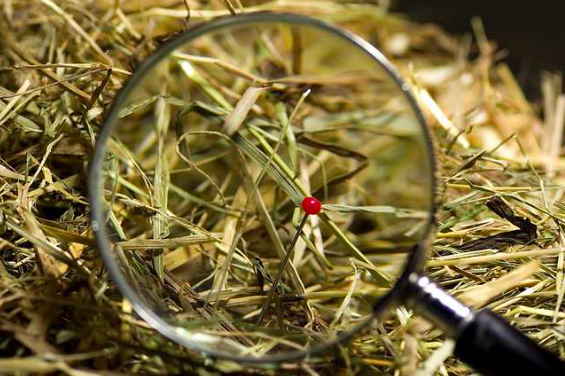
\includegraphics[scale=0.75]{pics/glass-needle.eps}
\end{center}

\subsection{Monitoring Pitfalls}
\vspace*{\fill}
\Huge
\begin{center}
Increasing the size of your haystack does not always
help in finding the needle. \\
\vspace{.4in}
Email is not a scalable network monitoring solution. \\
\vspace{.4in}
Absence of a signal can itself be a signal. \\
\vspace{.4in}
This list is incomplete.
\end{center}
\Normalsize
\vspace*{\fill}

\newpage
\vspace*{\fill}
\begin{center}
    \Hugesize
        Lecture 10 \\ [1em]
    \hspace*{5mm}
    \blueline\\
    \hspace*{5mm}\\
	System Security
\end{center}
\vspace*{\fill}

\subsection{How to determine {\em risk}}
``Risk Assessment''
\begin{itemize}
	\item identify {\em assets}
	\item identify {\em threats}
	\item identify {\em vulnerabilities}
	\item determine {\em likelihood of damage}
	\item estimate {\em cost of recovery}
	\item estimate {\em cost of defense}
\end{itemize}
\vspace{.5in}

A {\em risk} is the {\em likelihood} of a {\em threat} successfully exploiting
a {\em vulnerability} and the {\em estimated cost} (or potential damage) both
in the short and long term you may incur as a result.

\subsection{Threat Model}
For each system/component/product/service/...

\begin{itemize}
	\item identify {\em what} you're protecting
	\item identify {\em whom} you're protecting it {\em from}
		\begin{itemize}
			\item identify {\em goals} of the attacker
			\item identify {\em motivation} of the attacker
			\item identify {\em capabilities} of the attacker
		\end{itemize}
	\item identify threats you cannot defend against (within this
		system or in general)
\end{itemize}

\subsection{Cryptography}
Note:
\begin{itemize}
	\item {\em Authentication} \verb+!=+ {\em Authorization}
	\item cryptography does not handle authorization
	\item you generally need all three: confidentiality, integrity, authenticity
	\item cryptography cannot prevent against incorrect use \\
		(usability is hard, let's go shopping)
\end{itemize}
\addvspace{.5in}
Know your threat model!

\subsection{Secure by default}
\vspace{.5in}
\Huge
\begin{center}
Users care about usability, not about security. \\
\addvspace{.5in}
Users will not change their default settings. \\
\Normalsize
(Unless a less secure option is available.)
\end{center}

\subsection{Embrace Automation}
\vspace*{\fill}
\Huge
\begin{center}
	Vulnerabilities are dense. \\
\addvspace{.5in}
	Eliminate {\em classes} of attacks, not
	individual flaws. \\
\end{center}
\Normalsize
\vspace*{\fill}

\subsection{Build Robust Infrastructures and Service}
\vspace*{\fill}
\Huge
\begin{center}
	Your endpoint security model should assume the
	network is compromised; \\
	your network security model should assume the
	endpoint is. \\
\addvspace{.5in}
	Both in fact are.
\end{center}
\Normalsize
\vspace*{\fill}

\subsection{Threat Model}
\vspace*{\fill}
\Huge
\begin{center}
Your adversaries are determined human actors with
specific goals. \\
\addvspace{.5in}

Constantly seek to reduce your attack surface. \\
Identify and eliminate attack vectors.\\
\addvspace{.5in}

Don't be lazy.
\end{center}
\Normalsize
\vspace*{\fill}

\subsection{This Whole Semester in One Slide}
\vspace*{\fill}
\Huge
\begin{center}
Don't be lazy.
\end{center}
\Normalsize
\vspace*{\fill}

\end{document}
